\chapter{引言}
\label{cha:intro}

\section{研究背景}
\label{sec:background}

互联网的出现使人与人之间的交流变得简单轻松,信息交流更加便捷,各种各样的网络服务层出不穷,共享单车、网约车和在线教育就在很短的时间内让人们的生活发生了很大的改变。人们都在网上频繁获取信息,并寻找更加优质的服务。因此,它很大程度上改变了人们的生活方式,让人们的生活变得丰富多彩。第41次《中国互联网络发展状况统计报告》\footnote{http://cac.gov.cn/wxb\_pdf/CNNIC42.pdf}指出,截至 2018年6月,我国网民规模已达到了8.02亿,半年之内我国新增2968万网民,每天平均有近16万新网民加入互联网。互联网已经成为很多人工作生活中必不可少的一部分,不仅仅是人们生活中使用互联网的频率不断增加,很多企业也使用互联网管理设备和存储用户信息。
%互联网的出现使人与人之间的交流变得简单轻松,信息交流更加便捷,各种各样的网络服务层出不穷,共享单车、网约车和在线教育就在很短的时间内让人们的生活发生了很大的改变。人们都频繁在网上获取信息,并寻找更加优质的服务。因此,它很大程度上改变了人们的生活方式,让人们的生活变得丰富多彩。第41次《中国互联网络发展状况统计报告》\footnote{http://cac.gov.cn/wxb\_pdf/CNNIC42.pdf}指出,截至 2018年6月,我国网民规模已达到了8.02亿,半年之内我国新增2968万网民,每天平均几乎有16万新网民加入互联网,我国的互联网已经成为很多人必不可少的一部分。不仅仅是人们生活实用互联网频率不断增加,很多企业也使用互联网管理设备和存储用户信息。
%\footnote{http://cac.gov.cn/wxb_pdf/CNNIC42.pdf}

在这种情况下,发生网络安全问题就会对我们的社会造成极大的损失。2018年8月3日,台积电(TSMC)被Wannacry病毒入侵,它的基地生产线停摆。虽然最后病毒被成功清理,但是台积电也因此遭受约17.6亿元人民币损失。同年8月28日,华住酒店信息泄露,其中涉及姓名、身份证号、邮箱、家庭住址、开房记录等敏感信息约5亿条被出售。
%在这种情况下,网络安全问题就会对我们的社会造成极大的损失。有很多网络非法行为给人们造成了很多损失。2018年8月3日,台积电(TSMC)被病毒Wannacry病毒入侵,它的基地生产线摆停。虽然最后病毒被成功清理,但是台积电也因此预计造成约17.6亿元人民币损失。同年8月28日,华住酒店信息泄露,其中涉及姓名、身份证号、邮箱、家庭住址、开房记录等敏感信息约5亿条被出售。

因而,网络安全问题需要被重视,以减少网络安全问题造成的损失。在众多网络安全攻击中,拒绝服务(Denial of Service, DoS)攻击作为一种普遍而又威力强大的攻击,被黑客广泛地使用,对互联网的系统造成了极大的危害。而分布式拒绝服务攻击(Distributed Denail of Service, DDoS)作为DoS攻击的新模式,它拥有更加强大的攻击威力和更好的隐蔽性,使无数的企业都为该类攻击所困扰。


2018年1月29日, DDoS攻击迫使荷兰三大银行(荷兰银行、荷兰合作银行和ING银行)的服务器超载。因此,它们的网站和互联网银行服务瘫痪,荷兰税务局也遭受到类似的处境。
% http://www.sohu.com/a/272186665_100238920

2018年2月28日,世界上最顶尖的代码托管网站Github遭受了DDoS攻击并因此在几分钟内无法提供正常的服务,使很多公司都受到了影响。该攻击的峰值速率高达1.35Tb/s,超过了以往的所有DDoS峰值速率记录。
% http://www.sohu.com/a/272186665_100238920

2018年4月17日,美国的网络安全服务运营商Sucuri也遭受了大规模的DDoS攻击,导致一些端口的吞吐量达到容量上限,造成了非常高的延迟甚至还出现了数据包的丢失。因此,在西欧、南美和美国东部部分地区的服务被迫中断。
% http://www.cert.org.cn/publish/main/98/2018/20180426085352471430574/20180426085352471430574_.html

2018年5月13日,丹麦的铁路运营商(DSB)的系统受到了DDoS攻击,该公司的售票机、商店还有旅客的手机客户端都无法完成购票流程。因此,该公司不得不采用人工售票的方式暂时缓解压力,直到5月14日上午问题才得到解决。这次事件让1.5万旅客受到了影响。
%http://www.cert.org.cn/publish/main/98/2018/20180518143816118933026/20180518143816118933026_.html

如图\ref{fig:ddos_countries}所示,在卡巴斯基实验室2018年第四季度的调查\footnote{https://securelist.com/ddos-attacks-in-q4-2018/89565/}中,我国的网络安全形势不容乐观,中国依然是全世界范围内受DDoS攻击最严重的国家之一,因此,重视DDoS的防御问题是非常必要的。
% https://securelist.com/ddos-attacks-in-q4-2018/89565/

\begin{figure}
    \centering
    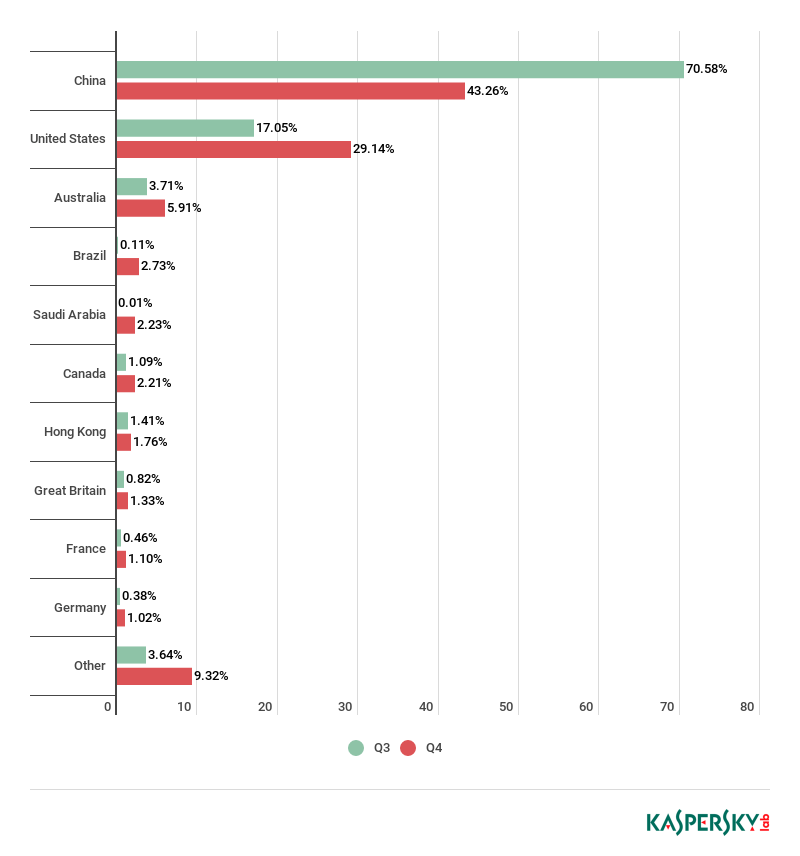
\includegraphics[scale=0.5]{figures/en-ddos-by-countries.png}
    \caption{在2018年Q3和Q4中,世界各国受DDoS攻击分布}
    \label{fig:ddos_countries}
\end{figure}

DoS攻击的危害性很大,而且它的实现形式也各不相同。在所有的DoS攻击种类中,低速率服务拒绝(Low-rate Denial of Service, LDoS)攻击\cite{LDoS}是一种针对良性TCP流最有效的一种攻击。和直接发送大量流量的洪泛方式不同,它仅通过发送周期性的脉冲低速流就可以持续迫使TCP流进入超时重传(Retransmission TimeOut,RTO)的等待阶段,造成TCP流吞吐量显著下降的可怕后果。而且由于LDoS攻击的平均速率很低,相对于洪泛方式的DoS攻击,LDoS攻击更加难以检测,而且,LDoS攻击以分布式方式实现的时候,LDoS攻击的隐蔽性更加强。
% Among all kinds of DoS attacks, the low-rate TCP attack~\cite{b20} is essentially the most efficient in terms of causing damage to benign TCP flows. Instead of directly sending a huge amount of traffic, it generates periodically pulsing low-rate flows to cause continuous retransmission of benign TCP flows, which results in significant throughput degradation. Due to the low rate, such attack is more difficult to be detected compared to flooding-based attacks. Moreover, the attack can be launched in a distributed mode, which further increases its stealthiness.

LDoS攻击对基于TCP协议发展起来的应用有非常大的影响,包括很多应用层的协议,例如BGP协议和HTTP协议。

有的研究\cite{b2}讨论了LDoS对BGP协议的影响。在使用LDoS攻击对运行BGP协议的网络进行干扰的情况下,BGP的控制平面误认为某条链路故障,导致该网络重新计算路径。因此,利用LDoS攻击可以迫使运行BGP协议的网络重复计算路径,不但会消耗控制平面的计算资源,甚至还会引发BGP的路由震荡。

有的研究\cite{Maci2007LoRDAS}针对HTTP协议提出了LDoS攻击的变种攻击LoRDAS。该类攻击能够以极小的代价就能持续占用HTTP的服务器队列资源,从而使正常的HTTP请求无法得到服务器的响应,给基于HTTP协议的网络造成极大的影响。


因此,由LDoS攻击引起的安全问题也受到了重视。目前,为了有效地防御LDoS攻击,很多相应的对抗方案已经被提出来。大部分的解决方案\cite{b1,b4, b6, b7, b22}通过使用数字信号处理(Digital Signal Processing, DSP)技术来提取频域特征。然而,只有采集数据流的周期合适的情况下,才能提取频域特征。而且,现行的方案都是采用一个固定的采样周期,来检测攻击流,这样会导致一些具有短周期的LDoS攻击流无法被检测出来。除此之外,这些方案都没有考虑限制被识别的攻击流的方法。有一些方案采用被动的防御方案来缓解LDoS攻击,不过,这些方案都没有识别攻击流,这些方案包括在主机上对TCP协议栈的RTO值进行随机化\cite{b17}和修改交换机上丢包机制的公平性规则\cite{b8}。这样的修改涉及到用户的网络协议栈或者交换机上面的硬件,因此这样的被动防御方案很难部署在大量的交换机上面。
%To effectively defend against the attack, several countermeasures have been proposed. Most defense solutions~\cite{b1,b4, b6, b7, b22} identify the attack flows by applying digital signal processing (DSP) techniques to extract frequency-domain characteristics. Such characteristics can only be well depicted when a proper sampling period of collecting flow statistics is set. However, existing methods apply a fixed sampling period, which may fail to detect attack flows with short periods. Besides, they do not consider how to throttle the identified flows. A few countermeasures adapt passive methods to mitigate the low-rate TCP attack without identifying attack flows, such as randomizing RTO of the TCP protocol stack in hosts\cite{b17} and modifying the fairness mechanism of dropping packets in the switches \cite{b8}. The passive defense solutions are not easy to be deployed in practice due to the modification of the network protocol stack in hosts or hardware in switches.

近来,软件定义网络(Software-Defined Networking, SDN)作为一个很有潜力的新型网络出现,改变了现行的网络架构的限制。首先,SDN网络将网络的控制平面从下层的路由器和交换机中分离出来,这样下层的交换机只需要负责数据平面,即转发数据流。其次,通过将数据平面和控制平面分离,SDN将控制逻辑放在中心控制器上,而交换机则负责数据的转发,这能够较为简单地配置网络和执行新的网络策略。而且,由于交换机只要与控制器完成连接,就可以接入已有网络并且不需要重复配置就能够执行统一的策略。



\begin{figure}
    \centering
    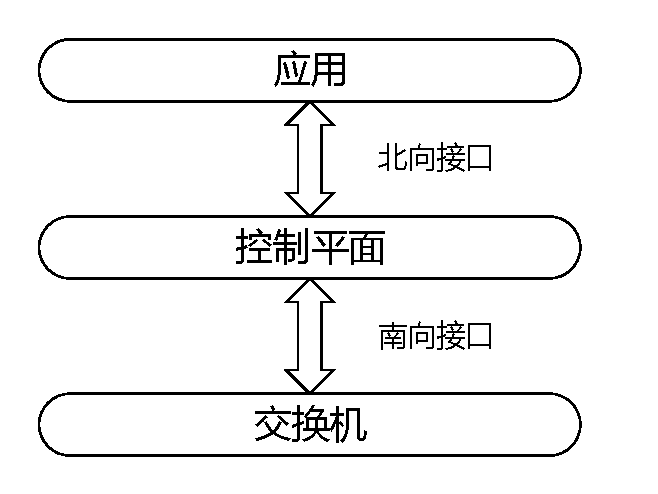
\includegraphics[scale=0.5]{figures/SDN-network}
    \caption{SDN网络架构}
    \label{fig:sdnfig}
\end{figure}

由于SDN是中心控制网络,控制平面和转发平面分离,通过编程灵活地制定网络安全策略能够达到比传统网络更加好的效果,所以,它在对抗DoS攻击上面有很多的优势。传统的网络设备上通过自身路由表项的字段识别DoS攻击。由于每个网络设备记录该设备信息,因此网络设备在某个端口处确认DoS攻击之后,需要上游的设备配合定位攻击源。但是,DoS攻击采用分布式的方式,很可能使防御系统在定位攻击源的时候丢失攻击源的信息。

因此,很多基于SDN实现的方案~\cite{b9, b16, b11, b23, b24}被提出来防御各种各样的DoS攻击。但是,已有的方案都将注意力集中在防御洪泛式的DoS攻击。他们都没有考虑到如何检测和缓解LDoS攻击。值得注意的是,LDoS攻击的攻击流特点与洪泛式攻击是有很大差别的。在SDN网络中,可以首先利用SDN独有的带宽限制机制在重要的链路上限制攻击流,接下来,利用SDN控制器对于全网的控制力来定位攻击源,直接对攻击源进行限制,从而达到防御LDoS攻击的效果。
%Recently, Software-Defined Networking (SDN) has emerged as a promising network paradigm. Due to the centralized control and flexible programmability, it shows great benefits on defeating DoS attacks. Several SDN-based approaches~\cite{b9, b16, b11, b23, b24} have been proposed to defend against various DoS attacks. However, existing defenses focus on defeating flooding-based DoS attacks. They fail to consider how to detect and mitigate the low-rate TCP attack. Now that the attack has great differences on the characteristics of the attack flows compared to the flooding attacks.


\section{主要研究内容}
\label{sec:work}
本文中的研究的主要内容是SDN网络的安全问题,针对DoS攻击的特殊攻击方式LDoS攻击的防御机制进行研究。在真实网络环境下,实现了两种基于SDN的LDoS攻击防御方案:基于带宽保障的方案和基于动态周期性检测的方案。两种方案在限制LDoS攻击上都有不错的表现。部署了防御方案的系统后,TCP流都不会因为LDoS攻击进入超时重传状态。同时,两种方案引入的开销也很低。本文在真实的SDN网络交换机上完成实验,并且对系统进行了评估。

本文首先介绍LDoS攻击防御的研究现状,然后对已有的SDN中的DoS攻击防御的研究进展进行讨论。接下来,本文通过分析LDoS攻击,针对其平均速率很低、瞬时速率很高、具有周期性的特点设计相应的防御方案,提出了两个方案来抵御LDoS攻击。第一种方案是基于带宽保障的方案,该方案通过Meter规则限制非TCP流的速率,保留了重要链路的TCP流所需要的带宽,不会让TCP流完全丢包;第二种方案是限制攻击源的方案,提出了基于周期性检测的LDoS攻击检测算法和基于平均欧氏距离(Mean Euclidean Distance, MED)的恶意流判定算法,再利用SDN的全局视野,可以找到攻击源,并对攻击源进行限制。第一种方案保障了重要链路的正常运行,该方案可以在LDoS攻击突发的时候,给TCP流保证部分带宽而让TCP流不会因为完全丢包而进入超时重传的长时间等待状态,直到LDoS攻击突发结束,TCP流重新恢复正常的传输,因此,LDoS攻击所造成的影响会小很多。第二种方案是使用两种算法精准地识别攻击流,然后利用SDN的全局视野,根据定位的攻击流直接安装相应的规则来限制攻击。若是LDoS攻击流的数据无法进入SDN网络,则LDoS攻击就无法对SDN网络造成任何影响,因此,使用第二种方案可以达到比已有的解决方案更加好的效果。


\section{研究意义}
\label{sec:contribution}
LDoS攻击防御的问题具有较大的研究意义。因为,在之前的工作中,传统网络的LDoS攻击的防御方案都有着其固有的缺陷:有的方案没有定位并且限制LDoS攻击源;有的方案需要对交换机或者主机进行比较大的修改,而且当新的设备接入网络的时候需要重新配置,相对比较复杂。且已有的SDN的DoS防御方案没有针对LDoS攻击的相关研究。相较于之前的LDoS防御方案,基于SDN的LDoS防御方案能够拥有更好的效果。总结本文的四个主要贡献点如下:

\begin{itemize}
    \item 本文综合分析了LDoS攻击的攻击原理,再分析了SDN的优势,提出了SDN中的防御系统,它能够有效地防御LDoS攻击而且不需要对交换机或者协议做任何修改。
    \item 本文提出了一种方案能够保证良性TCP流的基本传输,该方案能够使用Meter规则限制非TCP流的速率,保证了TCP流传输所需要带宽。所以,TCP流不会由于LDoS攻击而进入超时重传的等待时间。
    \item 本文提出了一种精准识别和限制LDoS攻击的方案。通过两个精准识别LDoS恶意攻击流的算法,能够准确地识别攻击源,并提出两种规则对被识别出的攻击流进行限制。
    \item 本文在真实的网络中,通过部署于Floodlight控制器上的LDoS防御系统,实现了单攻击源和分布式的LDoS攻击,验证了本文防御系统的有效性,并对两种方案进行了评估。
\end{itemize}

\section{各章内容安排}
\label{sec:arrange}
本文一共分为6章,各章节的主要内容如下:

第\ref{cha:intro}章的内容为引言,讲述了本文的研究背景,分析了已有方案对于LDoS防御的局限性,并提出了基于SDN的LDoS攻击防御方案,简要地分析说明了两种防御方案,并在最后总结了本文研究的意义。

第\ref{cha:relatedWork}章的内容为相关研究介绍,对目前LDoS攻击的相关防御工作的典型性方法进行分析,同时对SDN中DoS攻击的相关防御工作进行讨论。

第\ref{cha:LDoS}章主要介绍LDoS攻击的原理,分析LDoS攻击的特征,并且对LDoS的各种种类展开分析,最后对低速率分布式服务拒绝(Low-rate Distributed Denial of Service, LDDoS)攻击进行讨论。

第\ref{cha:design}章的主要内容为防御系统的设计,主要是设计两种LDoS攻击的防御方案,即带宽保障方案与LDoS攻击流限制方案。系统性分析两种方案的设计思想与对应的场景。

第\ref{cha:experiment}章的主要内容为实验总结和分析。在真实的SDN网络中,通过Floodlight分别部署两种方案的防御系统。在单攻击源和分布式LDoS攻击下,验证两种方案的有效性。最后,对比两方案的特点,同时对两个方案进行全方位比较和评估。

第\ref{cha:conclusion}章的主要内容为对本文的防御方案进行总结,并且对未来的工作进行探讨。